%%-------------------------------------------------------------------------------------- Início
\section{Controlador}
\begin{frame}[allowframebreaks, t, fragile]{Controlador}
	\begin{itemize}
		\item Um \alert{Action Controller} é classe Ruby contendo uma ou mais ações
		\item Cada \alert{ação} é responsável pela resposta a uma requisição
		\item Quando uma ação é concluída a \alert{visão} de mesmo nome é \alert{renderizada}
		\item Uma ação deve estar \alert{mapeada} no arquivo \alert{routes.rb}:
	\end{itemize}	
	\begin{figure}[h!]
		\centering
		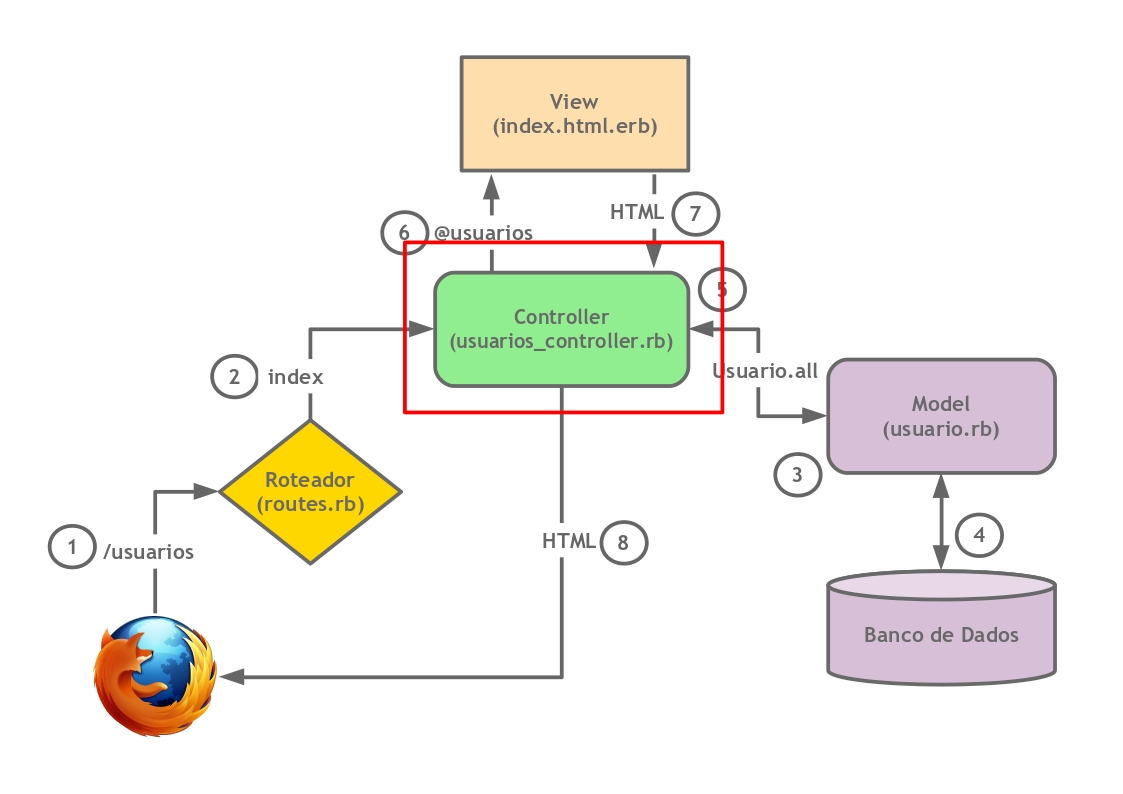
\includegraphics[width=0.80\textwidth]{imagens/mvc-controller.jpg}
	\end{figure}

\end{frame}